\documentclass{beamer}
\usepackage{tikz}
\usepackage{tikz-qtree}
\usepackage{gillius}
\usepackage{mathdots}
\usepackage{abraces}
\usepackage{etex}
\usepackage{array}
\usepackage[backend=biber]{biblatex}
\usepackage[export]{adjustbox}

% http://tex.stackexchange.com/questions/12703/how-to-create-fixed-width-table-columns-with-text-raggedright-centered-raggedlef
\newcolumntype{L}[1]{>{\raggedright\let\newline\\\arraybackslash\hspace{0pt}}m{#1}}
\newcolumntype{C}[1]{>{\centering\let\newline\\\arraybackslash\hspace{0pt}}m{#1}}
\newcolumntype{R}[1]{>{\raggedleft\let\newline\\\arraybackslash\hspace{0pt}}m{#1}}

\usetikzlibrary{external}
\usetikzlibrary{shapes}
\usetikzlibrary{arrows}
\usetikzlibrary{positioning}
\usetikzlibrary{decorations.pathreplacing}

\definecolor{blue0}{HTML}{EFF3FF}
\definecolor{blue1}{HTML}{BDD7E7}
\definecolor{blue2}{HTML}{6BAED6}
\definecolor{blue3}{HTML}{2171B5}

\usetheme[everytitleformat=regular]{m}
\setbeamertemplate{navigation symbols}{}
\setbeamercolor{background canvas}{bg=white}

\renewcommand\footnoterule{}

\title{Progress update: Phylogenetic inference of contact network parameters with kernel-ABC}
\author[RM \& AFYP]{Rosemary McCloskey and Art FY Poon}
\institute[UBC \& BCCfE]{BC Centre for Excellence in HIV/AIDS \\ University of British Columbia}
\date{February 1, 2016}

\newcommand{\dd}[2]{\frac{\text{d}\,#1}{\text{d}\,#2}}

\begin{document}

\maketitle

\begin{frame}{Table of contents}
\tableofcontents
\end{frame}

\section{Project overview}

\begin{frame}{Objective: network parameters from phylogenies}
  \begin{center}
  \vspace{-0.5cm}
  \begin{tikzpicture}
    [every node/.style={inner sep=2pt}]
    \node (t) {\includegraphics{figures/phylo}};
    \node [below=0 of t, text width=3cm, align=center] {observed \\ phylogeny};
    \uncover<2->{
      \node [left=of t] (t2) {\includegraphics{figures/tree2}};
      \node [above=0 of t2] (t1) {\includegraphics{figures/tree1}};
      \node [below=0 of t2] (t3) {\includegraphics{figures/tree3}};
      \node [below=0 of t3, text width=3cm, align=center] {simulated \\ phylogenies};
    }
    \node [left=of t1] (n1) {\includegraphics{figures/net1}};
    \node [left=of t2] (n2) {\includegraphics{figures/net2}};
    \node [left=of t3] (n3) {\includegraphics{figures/net3}};
    \node [below=0 of n3, text width=3cm, align=center] {contact network \\ model};
    \uncover<2->{
      \draw [->, >=stealth, very thick, color=blue1] (n1) -- (t1);
      \draw [->, >=stealth, very thick, color=blue2] (n2) -- (t2);
      \draw [->, >=stealth, very thick, color=blue3] (n3) -- (t3);
    }
  \end{tikzpicture}
  \end{center}
\end{frame}

\begin{frame}{Our work in context}
  \vspace{-0.5cm}
  \colorbox{blue0}{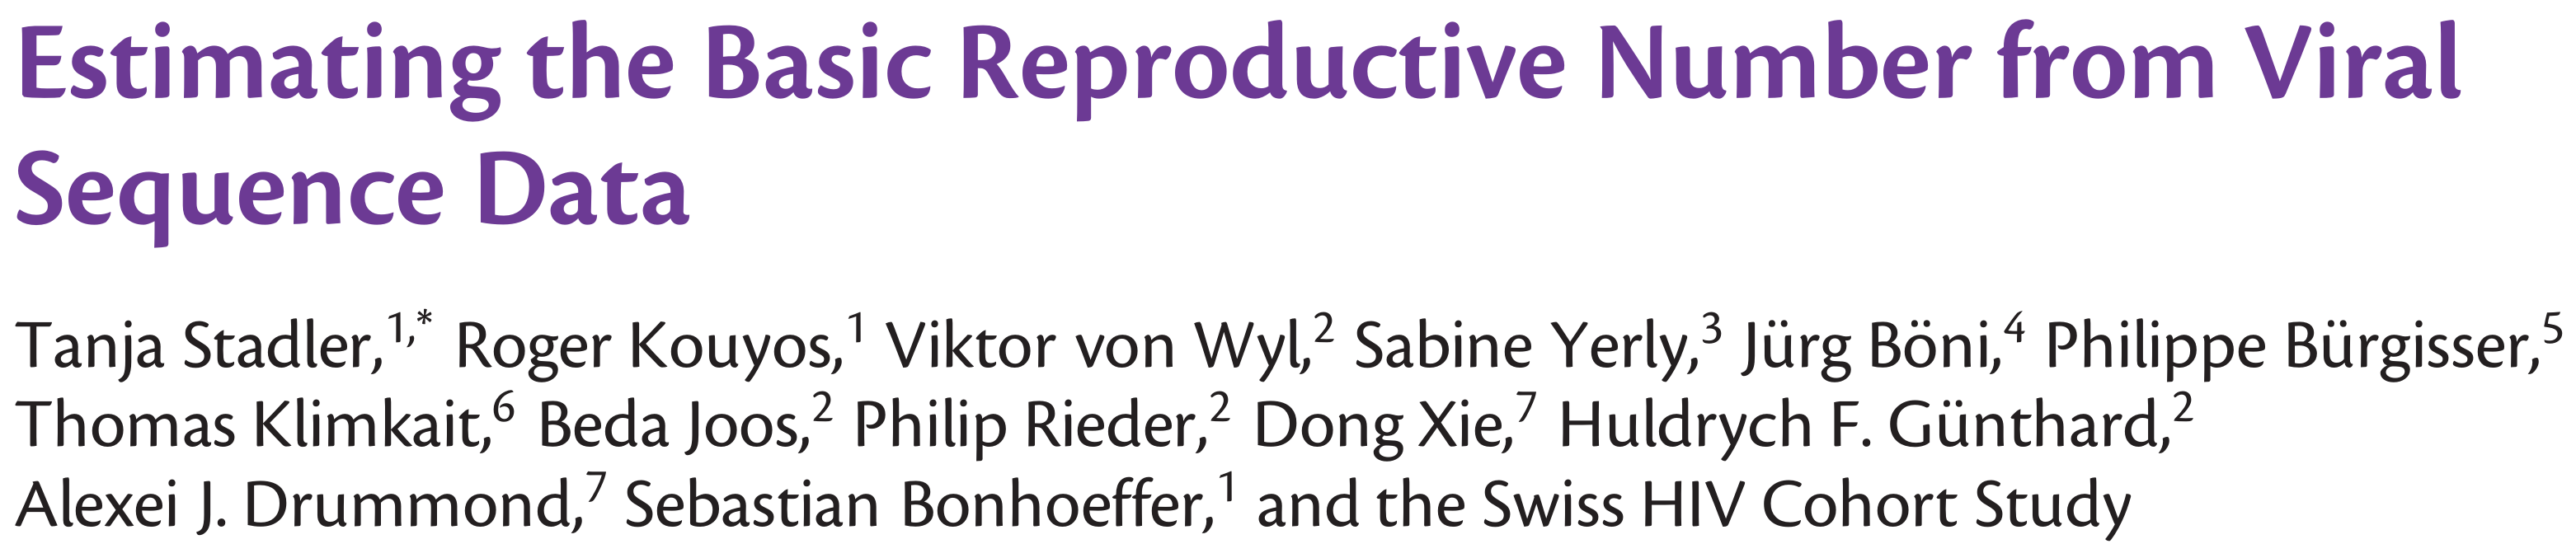
\includegraphics[width=\textwidth]{figures/stadler2011estimating}}

  \pause
  \colorbox{blue0}{
\includegraphics[width=\textwidth]{figures/leventhal2012inferring}}

  \pause
  \colorbox{blue0}{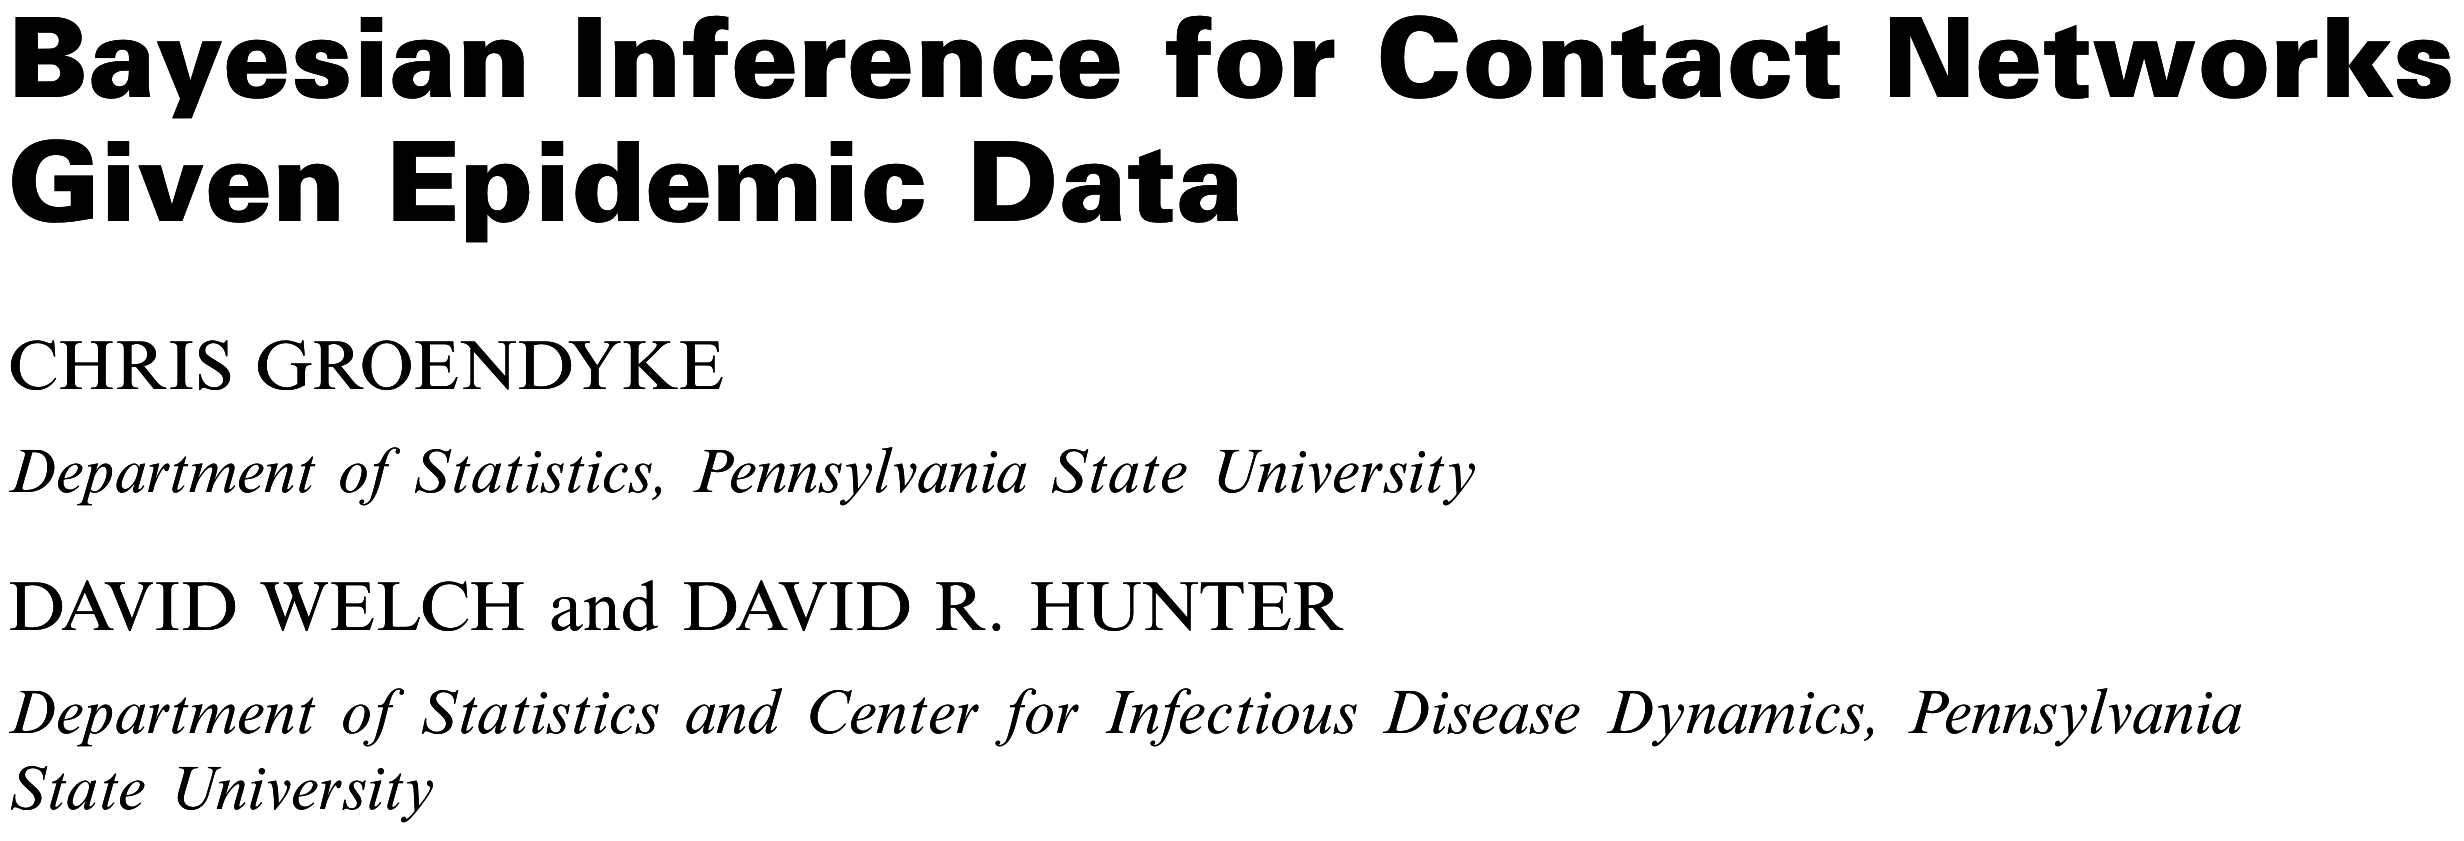
\includegraphics[width=0.75\textwidth]{figures/groendyke2011bayesian}}
\end{frame}

\begin{frame}{Parameter of interest: preferential attachment power $\alpha$}
  \vspace{-0.5cm}
  \includegraphics[height=0.9\textheight, center]{../thesis/figures/pa_power_bounds}
\end{frame}

\begin{frame}{Two similarity measures: nLTT and tree kernel}
  \begin{columns}
    \begin{column}{0.5\textwidth}
      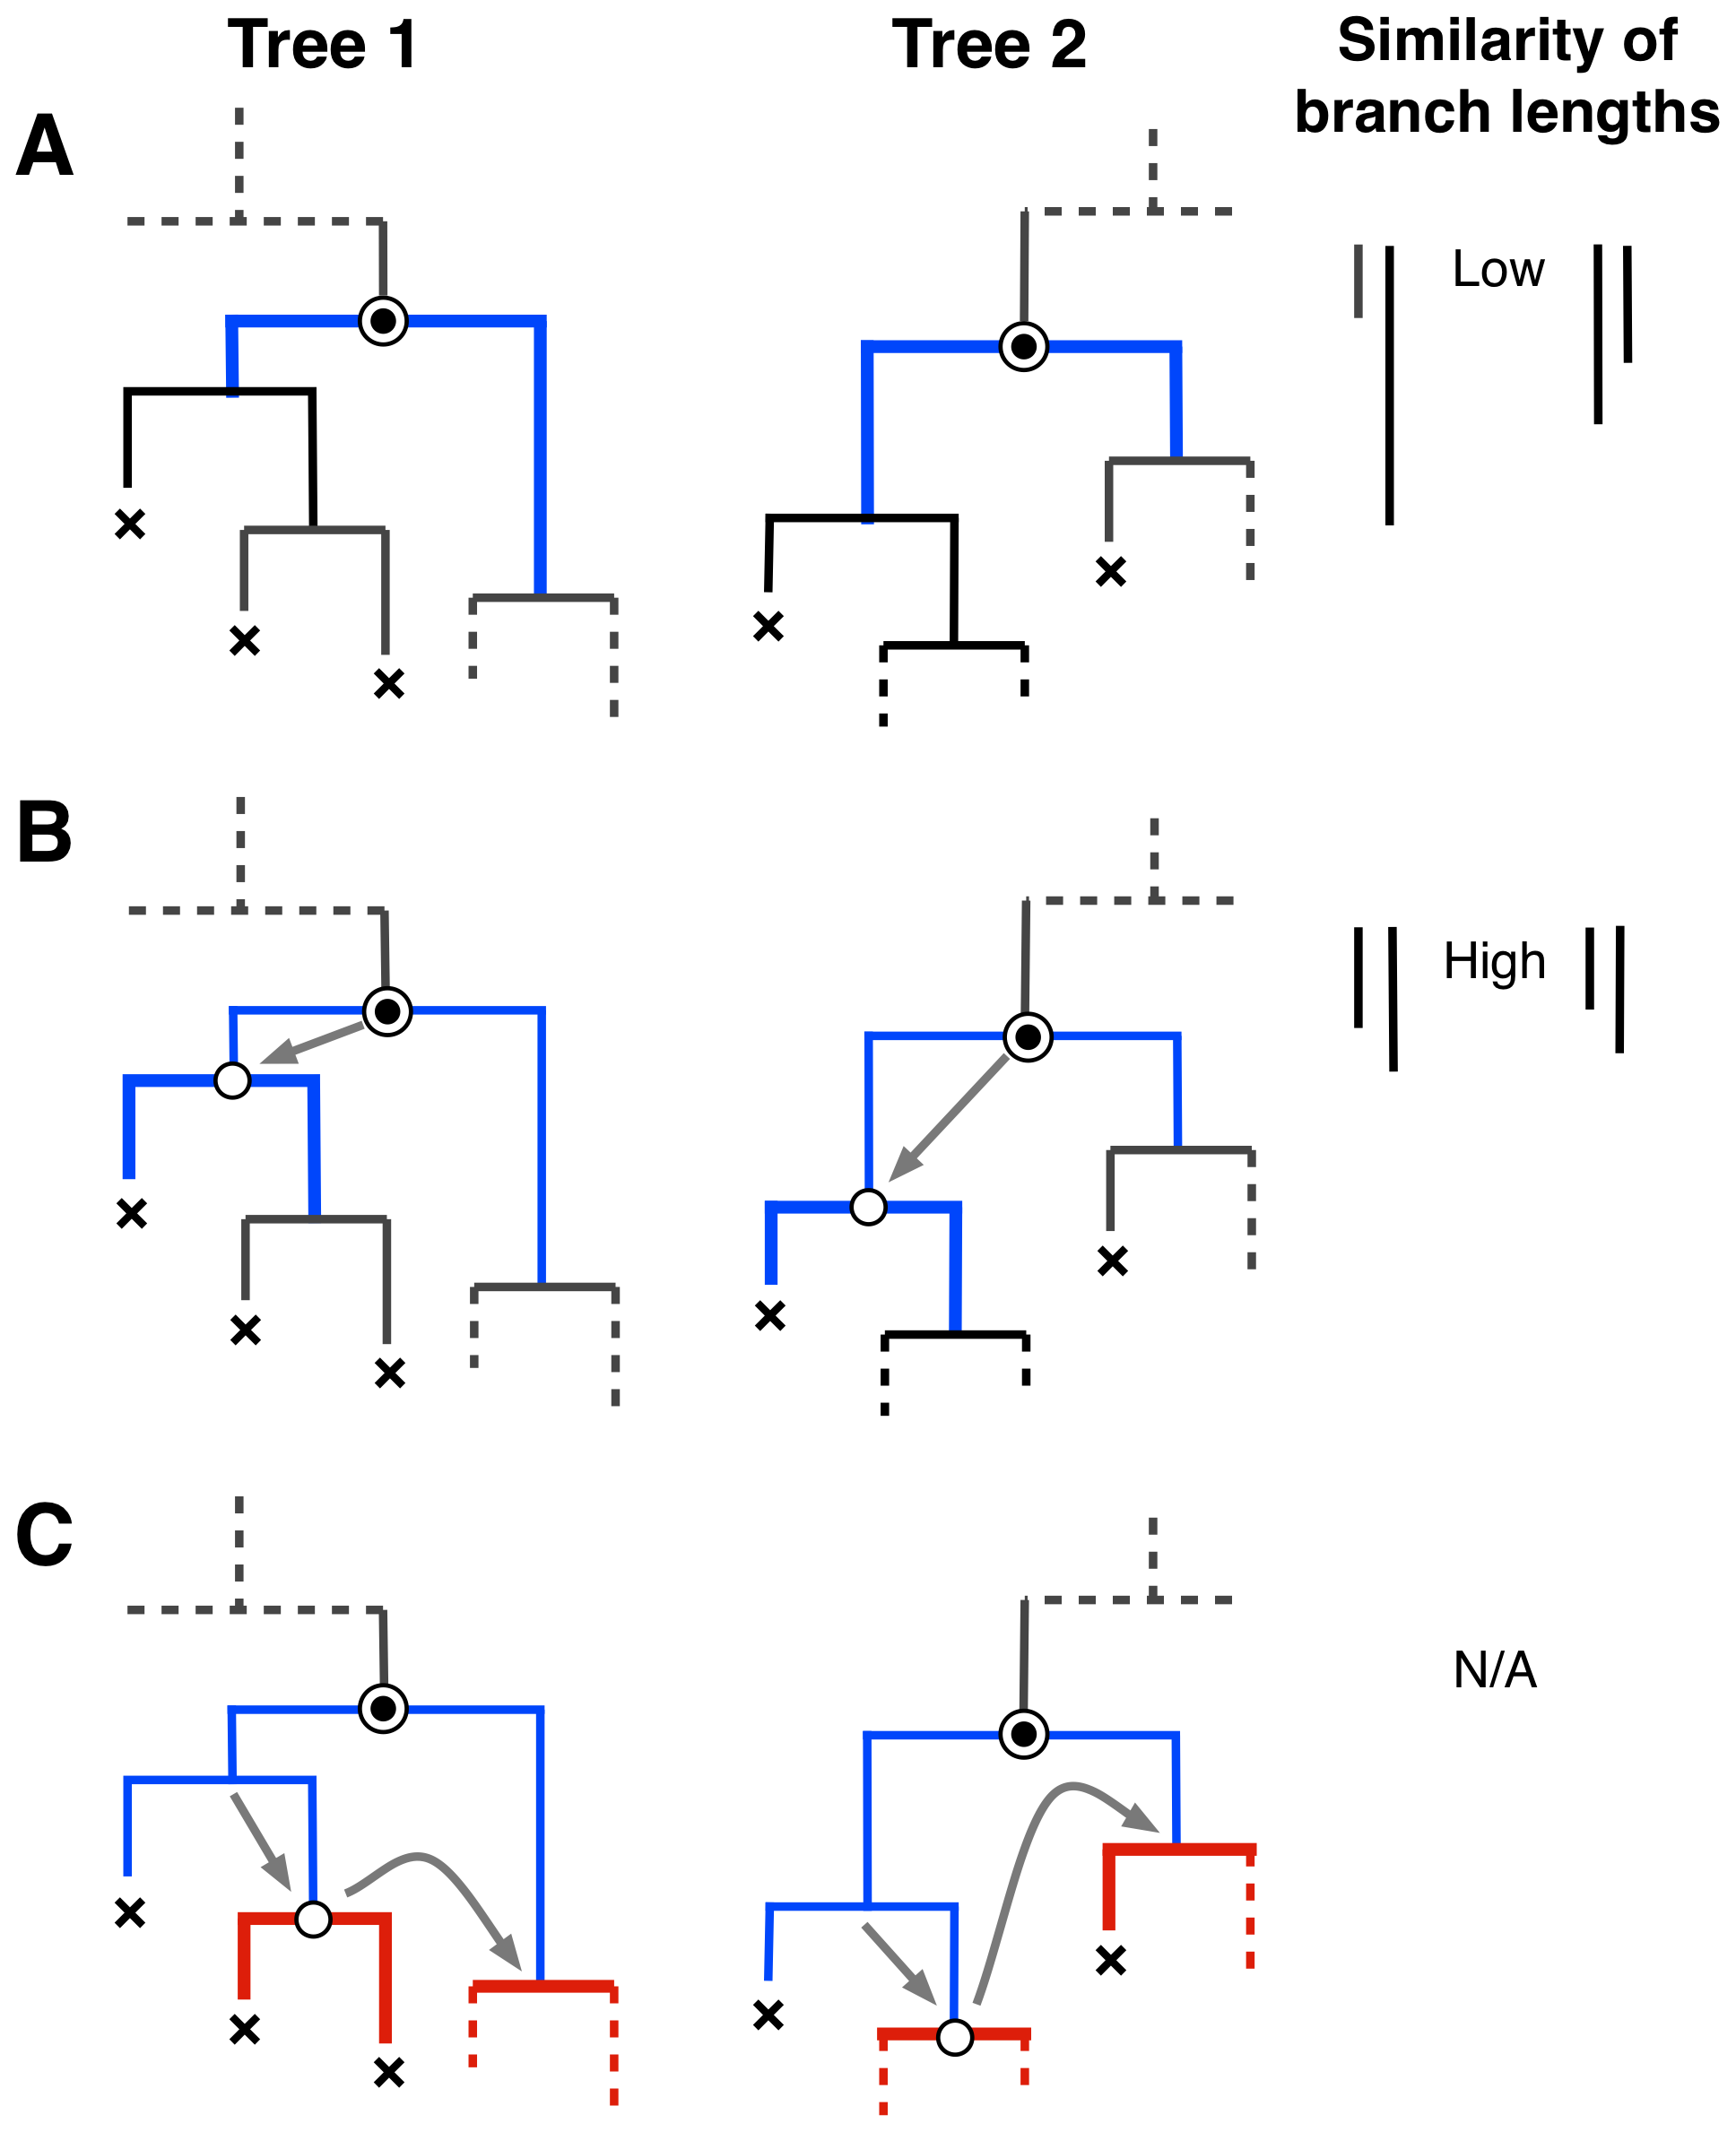
\includegraphics[width=0.9\textwidth]{figures/treekernel}
    \end{column}
    \begin{column}{0.5\textwidth}
      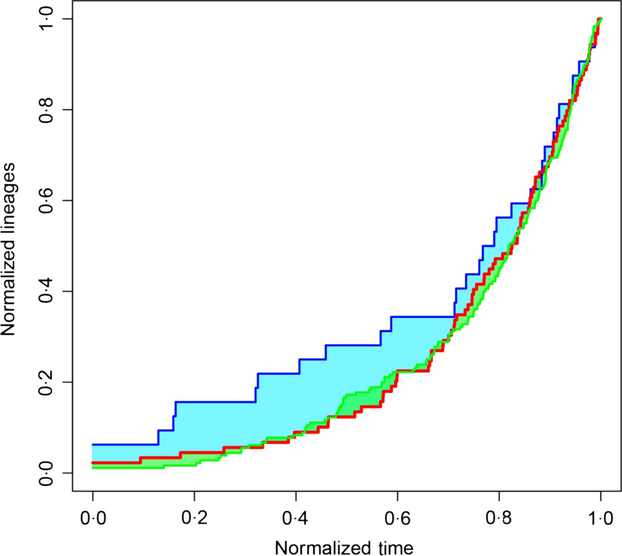
\includegraphics[width=0.9\textwidth]{figures/nltt}
    \end{column}
  \end{columns}
  \begin{columns}
    \begin{column}{0.5\textwidth}
      \tiny Poon, Art FY, et al. ``Mapping the shapes of phylogenetic trees
      from human and zoonotic RNA viruses.'' (2013): e78122.
    \end{column}
    \begin{column}{0.5\textwidth}
      \tiny Janzen, Thijs, Sebastian Höhna, and Rampal S. Etienne. ``Approximate
      Bayesian Computation of diversification rates from molecular phylogenies:
      introducing a new efficient summary statistic, the nLTT.'' Methods in
      Ecology and Evolution 6.5 (2015): 566-575.
    \end{column}
  \end{columns}
\end{frame}

\section{What's been done}

\subsection{Methods development}

\begin{frame}{Software}
  \textit{nettree:} simulate an epidemic over a contact network

  \begin{center}
    \includegraphics[scale=0.4, center]{figures/nettree}
  \end{center}
  \vspace{-0.5cm}
  \pause

  \textit{treekernel:} calculate the similarity of two trees
  \pause

  \textit{netabc:} infer contact network parameters from a phylogeny
\end{frame}

\begin{frame}{\textit{netabc} implements adaptive sequential Monte Carlo}
  \vspace{-0.5cm}
  \includegraphics[width=0.8\textwidth, center]{../thesis/figures/abc_smc.pdf}

  {\footnotesize Algorithm developed in: Del Moral, Pierre, Arnaud Doucet, and Ajay
  Jasra. ``An adaptive sequential Monte Carlo method for approximate Bayesian
  computation.'' Statistics and Computing 22.5 (2012): 1009-1020.}
\end{frame}

\subsection{Validation experiments}

\begin{frame}{Experiment 1: identify separable parameters}
  Trees simulated under different parameter values should segregate.

  \includegraphics[width=0.9\textwidth, center]{../thesis/figures/separable}
  \pause

  Use a kernel-SVM classifier to evaluate how well the values can be
  distinguished.
\end{frame}

\begin{frame}{Kernel-PCA to identify separable parameters}
  \includegraphics[width=0.9\textwidth, center]{../thesis/figures/kernel_expt}
\end{frame}

\begin{frame}{Trees with different attachment powers are distinctive}
  \vspace{-0.5cm}
  \includegraphics[width=1.1\textwidth, center]{figures/kernel-pa-tree}
\end{frame}

\begin{frame}{Higher attachment power $\Rightarrow$ more unbalanced trees}
  \vspace{-0.5cm}
  \includegraphics[height=0.9\textheight, center]{figures/kernel-pa-sackin}
\end{frame}

\begin{frame}{Attachment power is separable by the tree kernel}
  \vspace{-0.5cm}
  \includegraphics[height=0.9\textheight, center]{figures/kernel-pa-kpca}
\end{frame}

\begin{frame}{Tree kernel is more informative than Sackin's index}
  \vspace{-0.5cm}
  \includegraphics[height=0.9\textheight, center]{figures/kernel-pa-crossv}
\end{frame}

\begin{frame}{Prevalence parameter: sanity check on nLTT}
  Prevalence = how many nodes are infected before we stop the simulation.

  \includegraphics[width=\textwidth, center]{figures/prevalence}

  \begin{itemize}
      \pause
    \item Rate of new transmissions drops as network becomes saturated.
      \pause
    \item Prevalence should affect coalescence rate.
      \pause
    \item nLTT should be able to distinguish different coalescence rates.
  \end{itemize}
\end{frame}

\begin{frame}{Similar trees from different prevalence epidemics}
  \vspace{-0.5cm}
  \includegraphics[width=1.1\textwidth, center]{figures/kernel-nnode-tree}
\end{frame}

\begin{frame}{Tree balance is not associated with prevalence}
  \vspace{-0.5cm}
  \includegraphics[height=0.9\textheight, center]{figures/kernel-nnode-sackin}
\end{frame}

\begin{frame}{Prevalence is separable by the tree kernel}
  \vspace{-0.5cm}
  \includegraphics[height=0.9\textheight, center]{figures/kernel-nnode-kpca}
\end{frame}

\begin{frame}{Lineages-through-time is informative of prevalence}
  \vspace{-0.5cm}
  \includegraphics[height=0.9\textheight, center]{figures/kernel-nnode-crossv}
\end{frame}

\begin{frame}{Experiment 2: marginal parameter estimates}
  Grid search should be able to infer single parameters accurately when all
  others are fixed.

  \includegraphics[width=0.9\textwidth, center]{../thesis/figures/acc_prec}
\end{frame}

\begin{frame}{Grid search for marginal parameter estimates}
  \includegraphics[width=0.9\textwidth, center]{../thesis/figures/gridsearch_expt}
\end{frame}

\begin{frame}{Grid search precision depends on true $\alpha$ value}
  \vspace{-0.5cm}
  \includegraphics[height=0.9\textheight, center]{figures/gridsearch-pa-kernel}
\end{frame}

\begin{frame}{Accuracy varies for marginal estimates of $\alpha$}
  \vspace{-0.5cm}
  \includegraphics[height=0.9\textheight, center]{figures/gridsearch-pa-error}
\end{frame}

\begin{frame}{Experiment 3: full parameter estimates with ABC-SMC}
  Simulated trees under fixed parameter values; try to recover with ABC. 

  \begin{center}
    \begin{tabular}{ccc}
      \textbf{parameter} & \textbf{value} & \textbf{prior} \\
      \hline
      $\alpha$ & 0.0, 0.25, \ldots, 2 & Uniform(0, 2) \\
      $m$ & 2, 5, 8 & fixed \\
      $N$ & 5000 & Uniform(1000, 10000) \\
      $I$ & 1000 & Uniform(500, 2000) \\
      \hline
    \end{tabular}
  \end{center}
\end{frame}

\begin{frame}{ABC point estimates are accurate for $\alpha$, not $N, I$}
  \vspace{-0.5cm}
  \includegraphics[height=0.9\textheight, center]{figures/abc-pa-point}
\end{frame}

\begin{frame}{Priors on $N, I$ do not influence estimates of $\alpha$}
  \vspace{-0.5cm}
  \includegraphics[height=0.9\textheight, page=1, center]{figures/abc-pa-accuracy}
\end{frame}

\begin{frame}{Dispersion of posterior on $N$ depends on true $\alpha$}
  \vspace{-0.5cm}
  \includegraphics[height=0.9\textheight, page=2, center]{figures/abc-pa-accuracy}
\end{frame}

\begin{frame}{Dispersion of posterior on $I$ depends on true $\alpha$}
  \vspace{-0.5cm}
  \includegraphics[height=0.9\textheight, page=3, center]{figures/abc-pa-accuracy}
\end{frame}

\subsection{Real data analysis}

\begin{frame}{HIV in people who inject drugs in BC and China}
  \begin{center}
    \vspace{-1cm}
    \includegraphics[width=\textwidth]{figures/realtrees}

    \begin{tabular}{ccc}
      & BC & China \\
      \hline
      source & CfE & \footnote{\tiny Tee, Kok Keng, et al. ``Temporal and spatial dynamics of human immunodeficiency virus type 1 circulating recombinant forms 08\_BC and 07\_BC in Asia.'' Journal of virology 82.18 (2008): 9206-9215.} \\
      number of sequences & 399 & 314 \\
      known cluster & yes & no \\
      \hline
    \end{tabular}
  \end{center}
\end{frame}

\begin{frame}{BC: informative estimates for $\alpha$, not $N, I$}
  \vspace{-0.5cm}
  \includegraphics[height=0.9\textheight, center]{figures/bctree-posterior}
\end{frame}

\begin{frame}{China: estimating $m$ does not improve estimates of $N, I$}
  \vspace{-0.5cm}
  \includegraphics[height=0.9\textheight, center]{figures/cn-posterior}
\end{frame}

\begin{frame}{Higher attachment power in BC than in China}
  \vspace{-0.5cm}
  \includegraphics[height=0.9\textheight, center]{figures/bc_vs_cn}
\end{frame}

\section{Conclusions and future work}

\begin{frame}{Future work: more parameters; more real data}
  \vspace{-0.25cm}
  \colorbox{blue0}{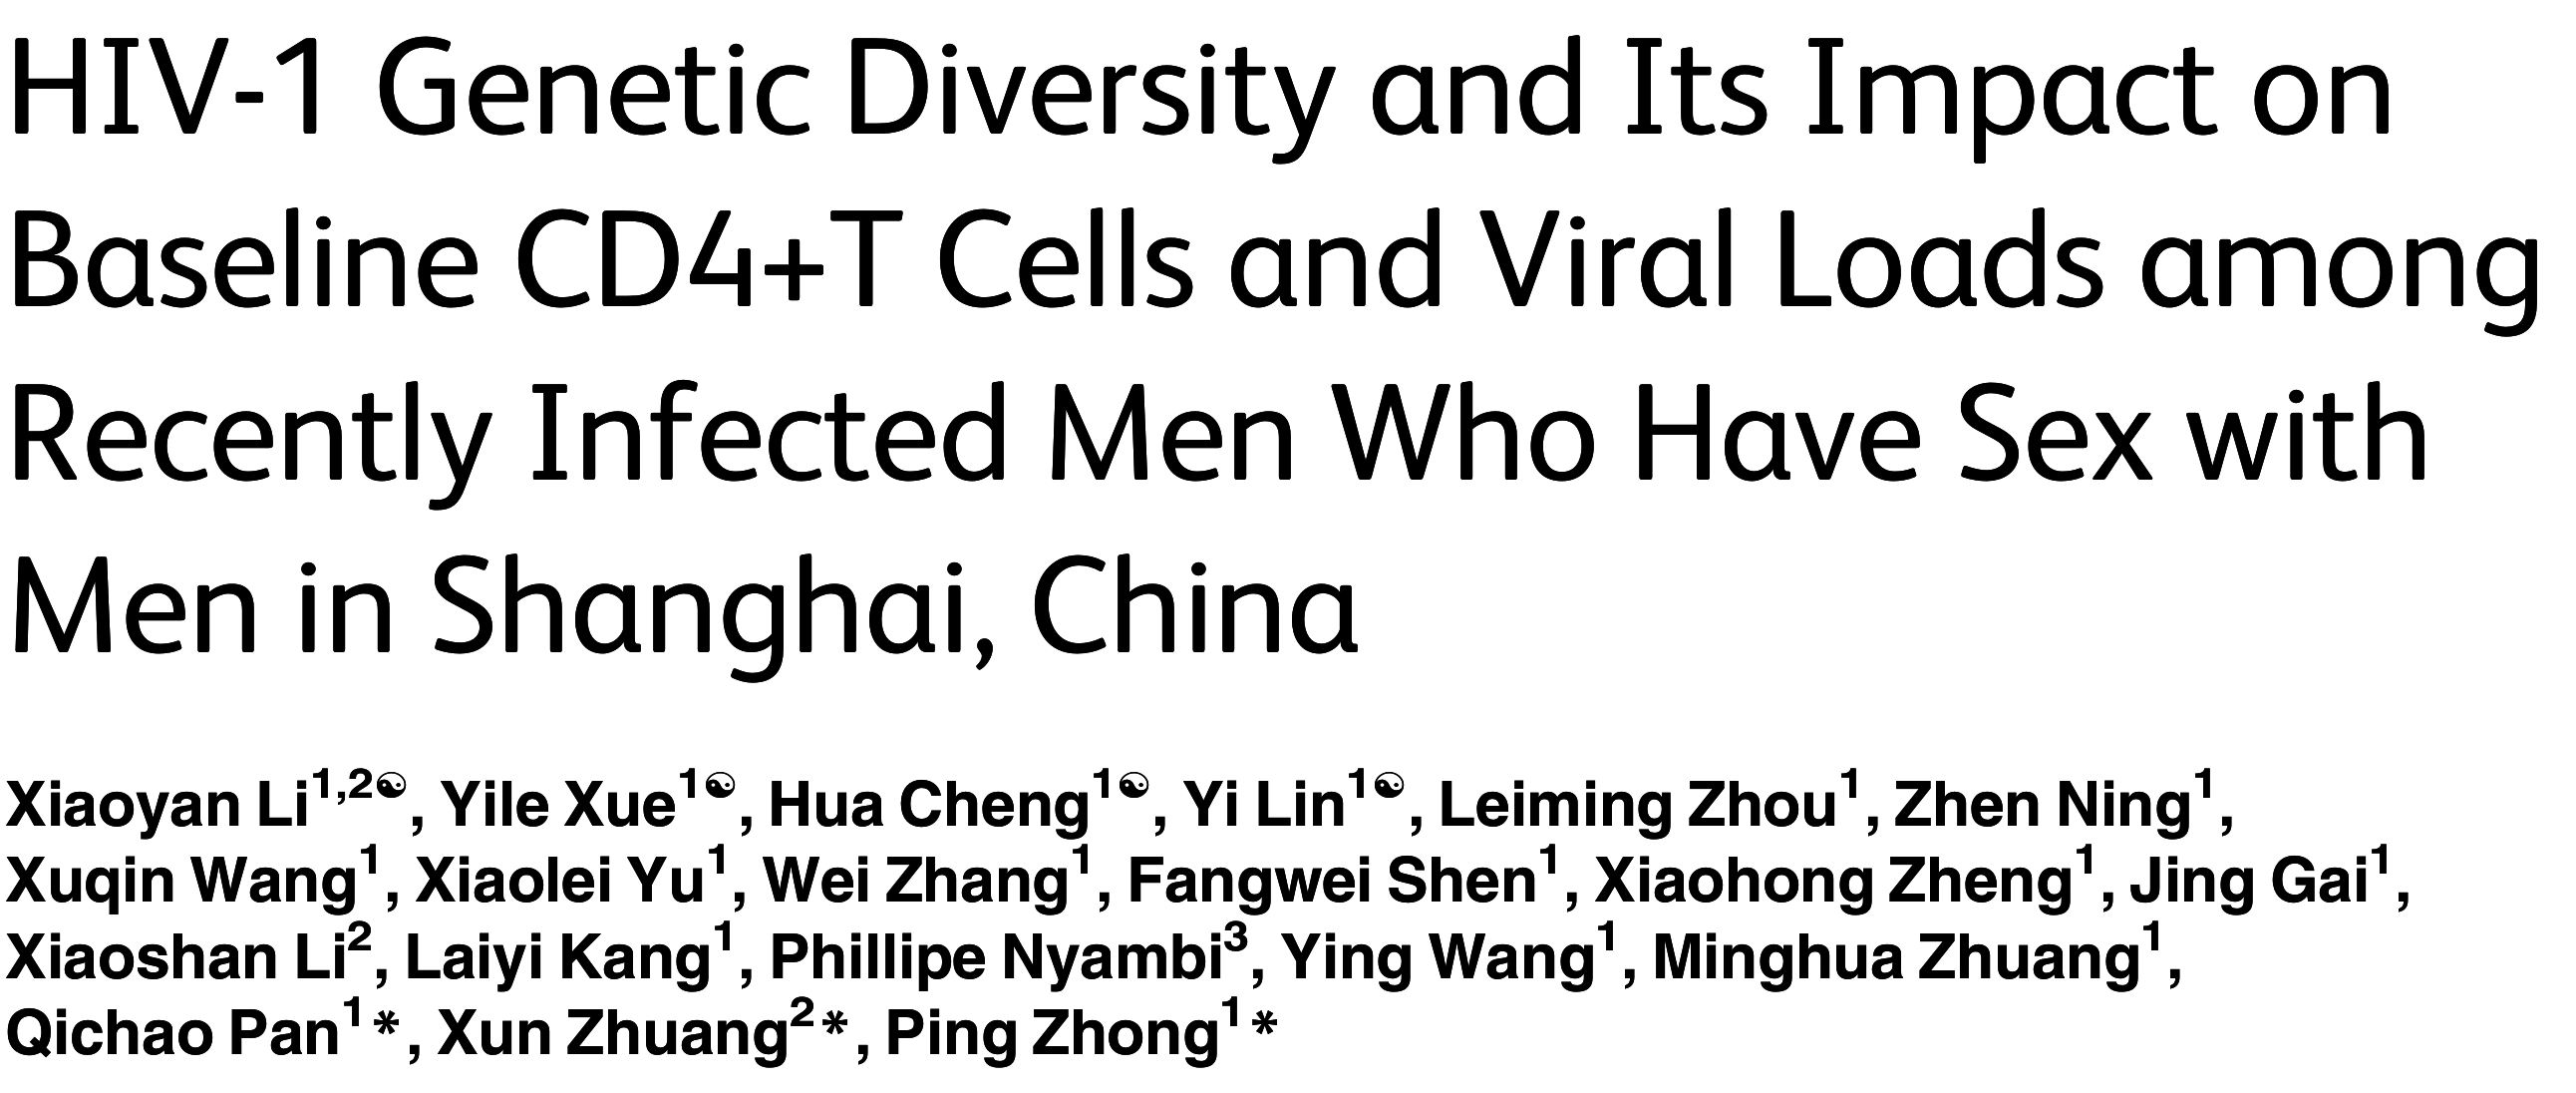
\includegraphics[height=2.7cm]{figures/li}}

  \colorbox{blue0}{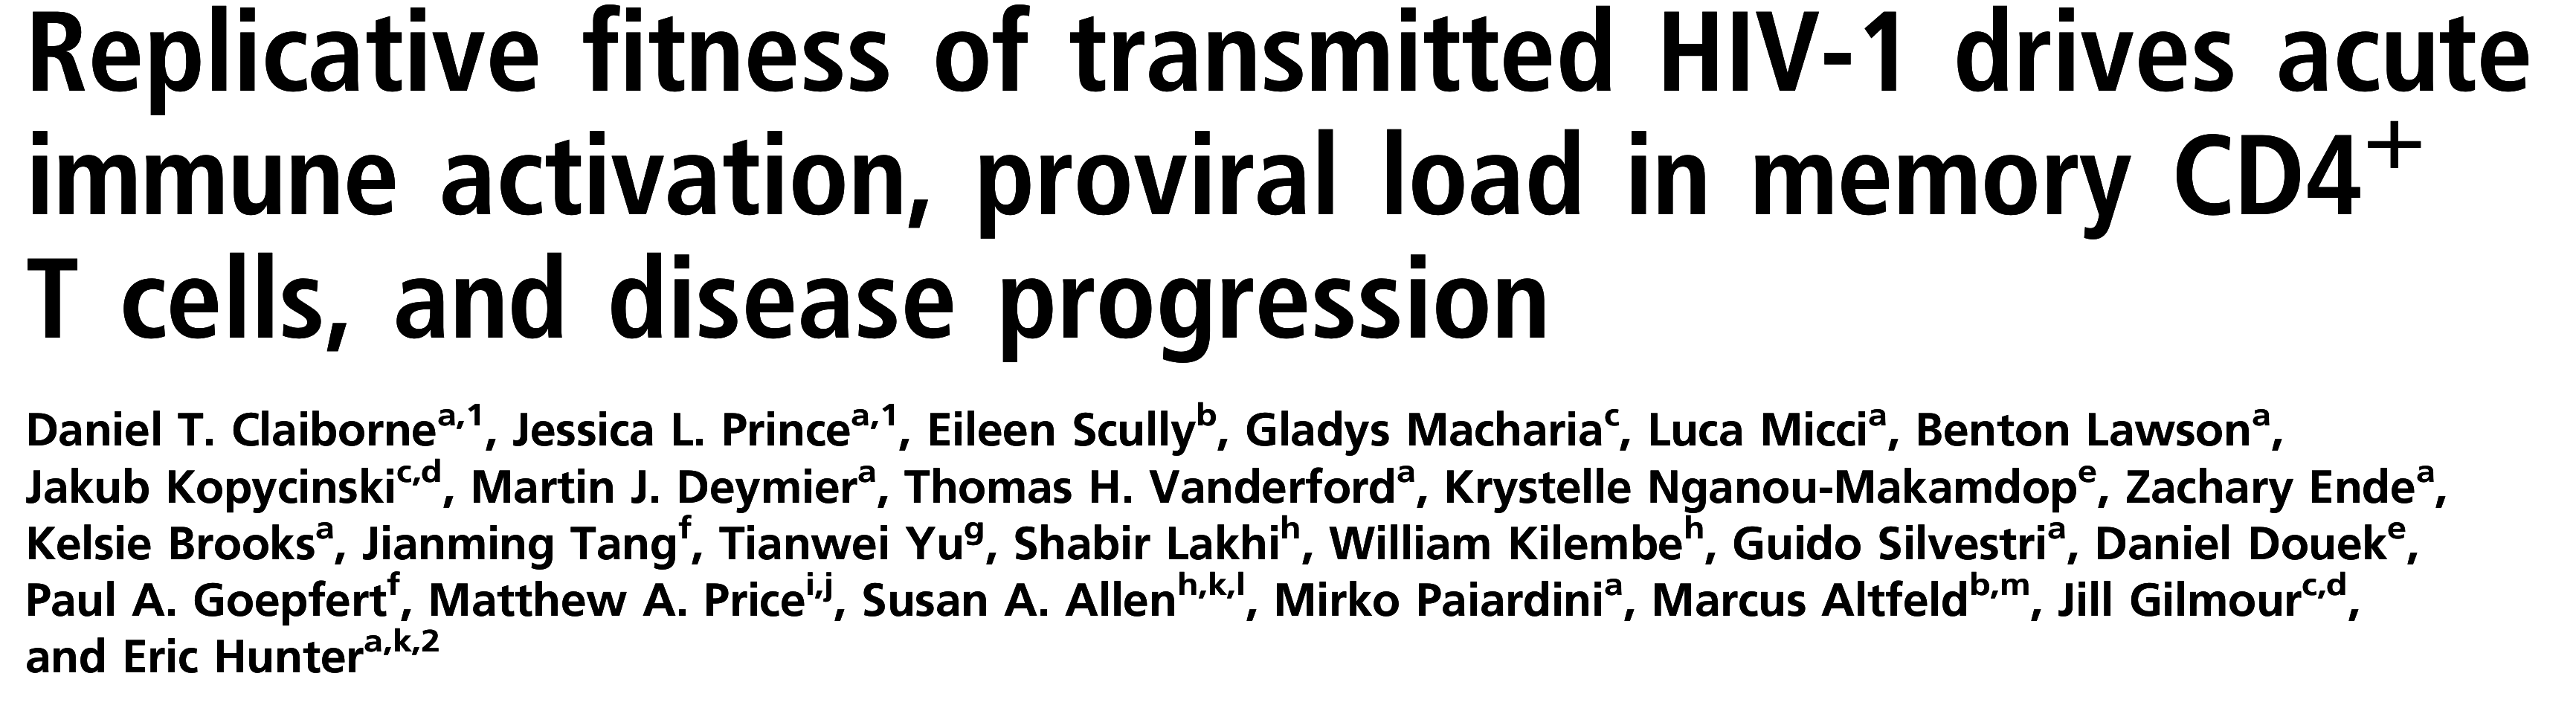
\includegraphics[height=2cm]{figures/claiborne}}

  \colorbox{blue0}{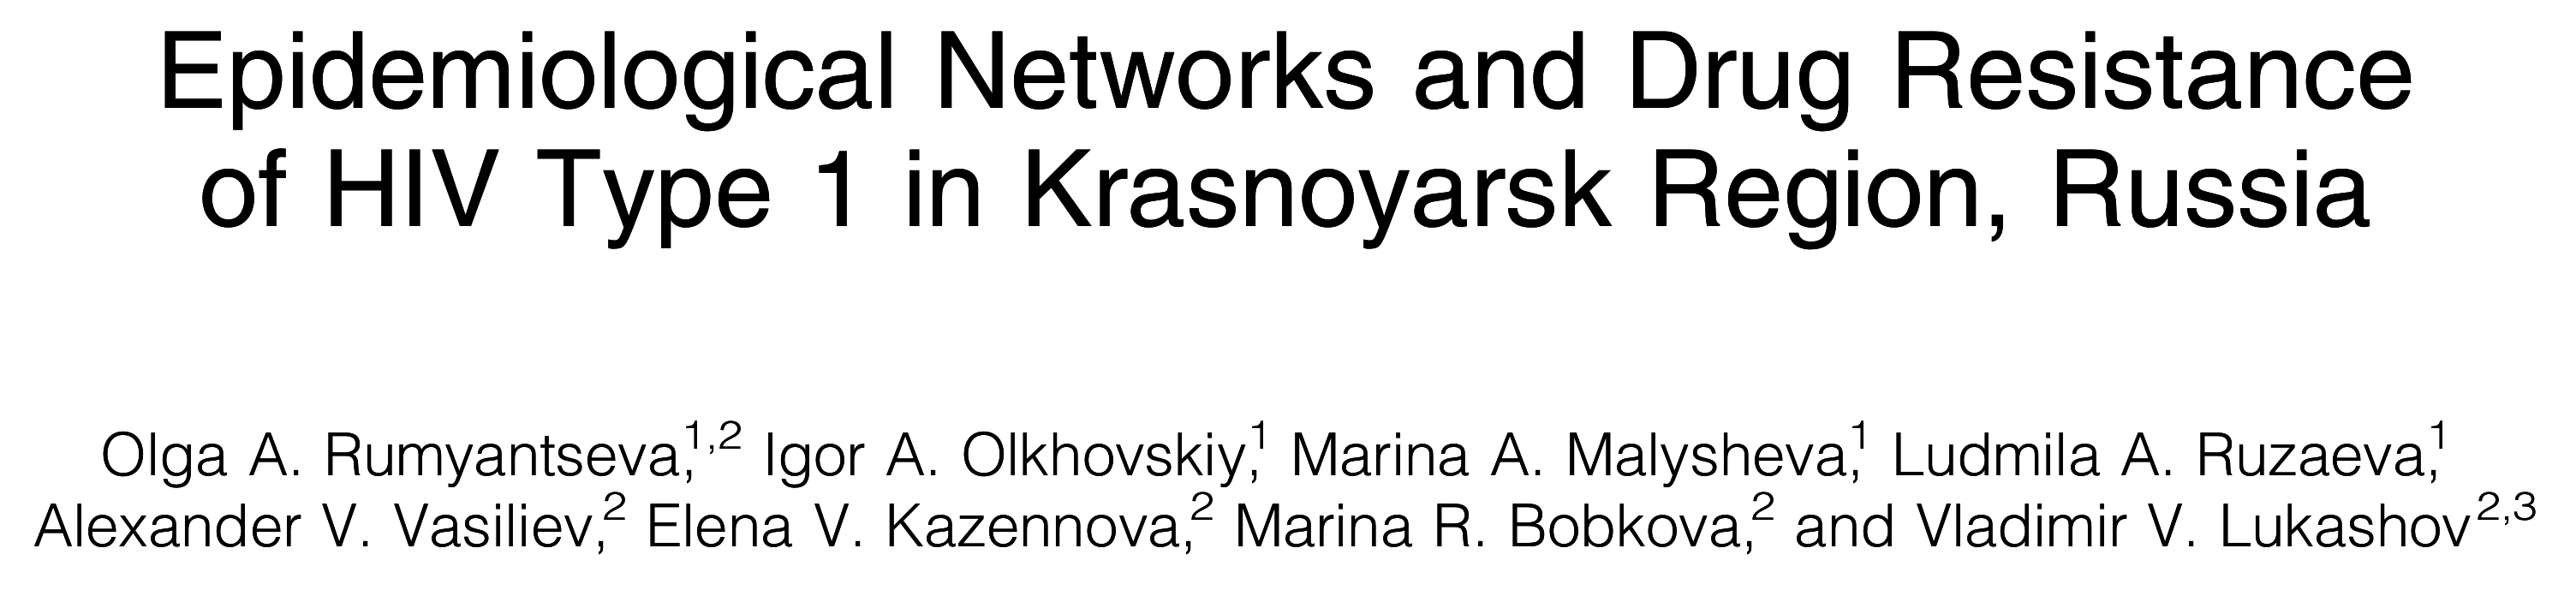
\includegraphics[height=2cm]{figures/rumyantseva}}
\end{frame}

\begin{frame}{Logos!}
  \vspace{-0.5cm}
  \begin{center}
  
\includegraphics[width=1in]{logos/btp}
  $\qquad$
  
\includegraphics[width=1in]{logos/cfe}
  $\qquad$
  
\includegraphics[width=1in]{logos/cihr}

  
\includegraphics[width=1in]{logos/genomebc}
  $\qquad$
  
\includegraphics[width=1in]{logos/msfhr}
  $\qquad$
  
\includegraphics[width=1in]{logos/phc}

  
\includegraphics[width=1in]{logos/phcri}
  $\qquad$
  
\includegraphics[width=1in]{logos/sphf}
  $\qquad$
  
\includegraphics[width=1in]{logos/westgrid}

  \includegraphics[width=0.5in]{logos/ubc}
  $\qquad$
  \includegraphics[width=1in]{logos/nserc}
  \end{center}
\end{frame}

\section{Appendix: clustering}

\begin{frame}{Appendix: replicating clustering in observed HIV tree}
  \vspace{-0.5cm}
  \includegraphics[width=\textwidth, trim=0 0 0 2cm, clip=true, center]{figures/pcbr}
\end{frame}

\begin{frame}{Cliques with baseline rate do not give similar trees}

  \begin{columns}
    \begin{column}{0.5\textwidth}
      \includegraphics[width=\textwidth, trim=0 0 0 1.5cm, clip=true]{figures/net20}
    \end{column}
    \begin{column}{0.5\textwidth}
      \includegraphics[width=\textwidth, trim=0 0 20cm 4cm, clip=true]{figures/tree20}
    \end{column}
  \end{columns}
\end{frame}

\end{document}
